\documentclass[a4paper,10pt]{article}
\usepackage[utf8]{inputenc}
\usepackage[english,russian]{babel}
\usepackage[top=2cm,bottom=3cm,left=0.5cm,right=2cm,nohead]{geometry}
\usepackage{multicol}
\usepackage{graphicx}
\usepackage{tabularx}

\graphicspath{{images/}}

\begin{document}
\section*{Шпора по околобесполезной херне}
приницпы фон Неймана: \\
\begin{enumerate}
    \item принцип двоичного кодирования
    \item принцип адресности - Все ячейки ОП имеют фиксированный размер, который называется машинным словом, также все ячейки пронумерованы, номер ячейки является её адресом
    \item принцип программного управления
    \item принцип последовательного исполнения
    \item принцип однородности
\end{enumerate}
cisc - complex instruction set computer \\
risc - reduced instrucrion set computer \\
\begin{figure}[htbp]
    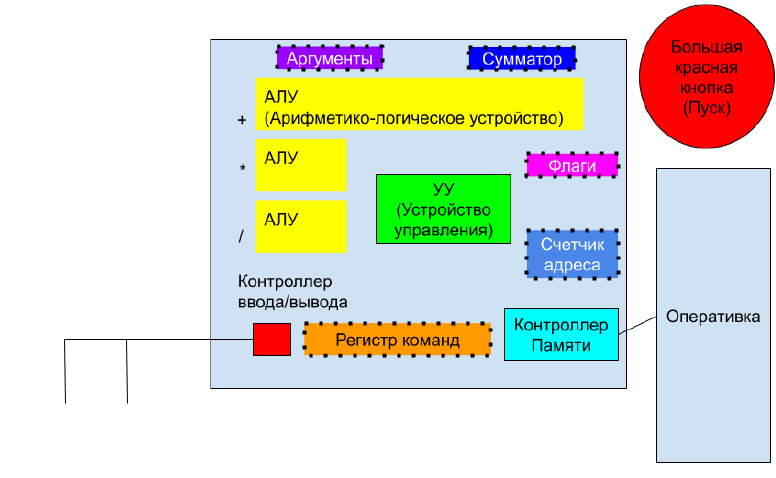
\includegraphics[width=0.8\textwidth]{УМвид.png}
\end{figure} \\
цикл работы УМ
\begin{enumerate}
    \item[0] инциализация
    \item[1] считывание команды
    \item[2] декодирование команды
    \item[3] считывание аргументов из ОП
    \item[4] выполнение в сумматора АЛУ
    \item[5] запись в ОП
    \item[6] увеличение счётчика переход на 1 пункт 
\end{enumerate}
\begin{tabularx}{\textwidth}{|X|X|X|X|X|}
    \hline
    соглашение & параметры регистры & параметры стек & чистит стек & имя \\
    \hline
    stdcall & нет & справо-налево & вызываемый & \_<имя>[@N] \\
    \hline
    cdecl & нет & справо-налево & вызывающий & \_<имя> \\
    \hline
    fastcall & ecx,edx & справо-налево & вызываемый & @<имя>[@N] \\
    \hline
    pascal & нет & слева-направо & вызываемый & <имя> капсом \\
    \hline
    register* & eax,edx,ecx  & слева-направо & вызывающий & (нет) \\
    \hline
\end{tabularx} \\
\\
\begin{tabularx}{\textwidth}{|c|X|c|c|X|c|c|X|}
\hline
7&6&5&4&3&2&1&0 \\
\hline
extrn&операнд в стеке&определён&регистр&перемещаемый адрес&констнанта&область данных&метка процедура \\
\hline
\end{tabularx}
редко используемое: lock, clwb (cache line write back), clflush, sfence (store), lfence (load), mfence (s \& l), prefetch[012], movntxx, int, iret. \\
\begin{tabularx}{\textwidth}{|X|X|X|X|X|X|}
    \hline
    1&2&3&4&5&6 \\
    \hline
    Выбор команды&Декодирование&вычисление адресов&выбор операндов&выполнение&запись \\
    \hline
\end{tabularx}
строковые операции: cmps[], movs[], scas[] (edi), lods[] (esi), stos[] (edi)
\begin{tabular}{|c|c|}
    \hline
    cld & DF:=0 строковые операции на увеличение адресов \\
    std & DF:=1 строковые операции на уменьшение адресов \\
    clc & CF:=0 \\
    stc & CF:=1 \\
    cmc & CF:=not(CF) \\
    cli & IF:=0 Interrupt Flag замаскировать прерывания (кроме №2) прерывания будут игнорироваться \\
    sti & IF:=1 Interrupt Flag вернуть обычное поведение с прерываниями \\
    lahf & загрузить в \textbf{ah} арифметические флаги AH := EFLAGS(SF,ZF,0,AF,0,PF,1,CF)\\
    sahf & загрузить из \textbf{ah} арифметические флаги EFLAGS(SF,ZF,0,AF,0,PF,1,CF) := AH\\
    pushfd & загрузить в стек 32 рязрядный EFLAGS \\
    popfd & забрать 32 разрядный EFLAGS \\
    \hline
\end{tabular}
\end{document}